\chapter{Lecture 28 - Solving Boundary value Problems Using the Shooting Method}
\label{ch:lec28n}
\section{Objectives}
The objectives of this lecture are to:
\begin{itemize}
\item Review basic concepts for Boundary Value Problems with a single independent variable.
\item Describe the Shooting Method.
\item Do an example problem.
\end{itemize}
\setcounter{lstannotation}{0}

\section{Boundary Value Problems}
A boundary value problem (BVP) consists of a governing equation and boundary conditions.  For a second-order boundary value problem with one spatial dimension\sidenote{Here we assume that the independent variable is a \emph{spatial} variable.  This is the conventional approach for applications of interest for this class.}, the governing equation is as given in Equation \ref{eq:lec28n-bvp-gov-eq}:
\begin{equation}
\frac{d^2 u}{dx^2} = f\left(x,u,\frac{du}{dx}\right), \ \ a\le x \le b
\label{eq:lec28n-bvp-gov-eq}
\end{equation}
where it is understood that $a<b$.  

In order to obtain a unique solution, suitable boundary conditions must be provided.  Linear boundary conditions for the second-order problem take the form shown below:
\begin{align*}
A_1u(a)+B_1u^{\prime}(a)&=C_1 \\
A_2u(b)+B_2u^{\prime}(b)&=C_2
\end{align*}
where $A_i$, $B_i$, and $C_i$ are constants and are not \emph{all} zero for any value of $i$.

\newthought{Knowing what constitutes} a \emph{suitable} set of boundary conditions is part of your job as an engineer.  Depending on the given boundary conditions, the BVP may have one unique solution, no solution, or infinitely many solutions. Somtimes it is hard to tell in advance which of these will turn out to be the case.  Physical insight and intuition can play an important role in predicting these outcomes so it is essential that one understands the physical interpretation of a proposed set of boundary conditions.

There are three basic types of boundary conditions:\marginnote{\textbf{Note:}This classification scheme is also discussed in Lecture 22 of the Analytical Methods portion of this text.}
\begin{itemize}
\item \textbf{Type 1} or \emph{Dirichlet} boundary conditions.  For this type of boundary condition, the value of the dependent variable is directly fixed on the boundary.  For example:
\begin{equation*}
u(a) = 100
\end{equation*}
For a BVP related to the heat equation, for instance, this is equivalent to specifying the temperature on a boundary.
\item \textbf{Type 2} or \emph{Neumann}\sidenote{Here we refer to Carl Gottfried Neumann who was a German mathematician in the late 19th and early 20th century.  He taught at several universities and carried out research in pure and applied mathematics.  There are several other mathematical terms named after him including the Neumann series, the Neumann boundary value problem and the Neumann-Poincar\'e operator.  } boundary conditions.  For this type of boundary condition, the derivative of the dependent variable is directly fixed on the boundary.  For example:
\begin{equation*}
\frac{du}{dx}\Bigl|_{x=b} = 0
\end{equation*}
For a BVP related to the heat equation where the dependent variable is temperature, this is equivalent to specifying the heat flux on a boundary.  For the example given, if we set the heat flux equal to zero, that is interpreted as an \emph{insulated} boundary condtion.

\item \textbf{Type 3} or \emph{Robin}\sidenote{Named for Victor Gustave Robin who was a French matematician who lectured at the Sorbonne in Paris. To the best of this author's knowledge, he was not associated in any way with Batman.} or just \emph{mixed} boundary conditions. As the reader may have deduced by now, boundary conditions of this type involve both the dependent variable and its derivative.  For example:
\begin{equation*}
\frac{du}{dx}\Bigl|_{x=a} = -h\left(u(a) - T_{\text{env}}\right)
\end{equation*} 
where $T_{\text{env}}$ refers to the environmental temperature near the boundary and $h$ is a non-negative constant. This example corresponds to heat transfer by convection.  The constant $h$ is the convective heat transfer coefficient and relates heat flux at the boundary to the difference between the temperature at the boundary of the domain ($u(a)$) and $T_{\text{env}}$.  In the limit of $h\to 0$, the boundary becomes insulated.

\end{itemize}

\section{The Shooting Method}
We will introduce and illustrate our first method for solving BVPs, the shooting method, with an example.

\vspace{0.25cm}

\noindent\textbf{Problem Statement:}

\vspace{0.1cm}

\noindent A pin fin is a slender extension attached to increase the surface area and enable greater heat transfer.  When convection and radiation are included in the analysis, the steady-state temperature distribution, $T(x)$, along a pin fin can be caluclated from the solution of the equation below:
\begin{equation}
\frac{d^2T}{dx^2} - \frac{h_cP}{kA_c}\left(T - T_s\right)-\frac{\epsilon \sigma_{SB}P}{k A_c}\left(T^4 - T_s^4 \right) = 0, \ \ 0 \le x \le 1
\end{equation}
with boundary conditions $T(0)=T_A$ and $T(0.1)=T_B$.  A schematic of the system is shown in Figure \ref{fig:lec28n-ex1-schematic}.  There are a number of parameters given in the equation.  These are specified in Table \ref{tab:lec28n-ex1-parameters}.
\begin{marginfigure}[-4.5cm]
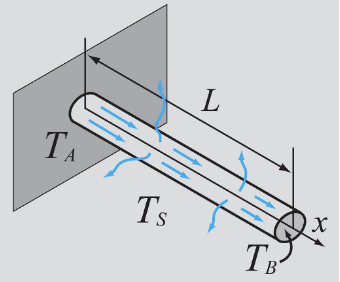
\includegraphics{lec28n-ex1-schematic.png}
\caption{Pin Fin Boundary Value Problem Schematic.}
\label{fig:lec28n-ex1-schematic}
\end{marginfigure}

\begin{table}
\begin{tabular}{|c|c|}
\hline
\textbf{Parameter} & \textbf{Value} \\ \hline
Convective heat transfer coefficient ($h_c$) & 40 $\text{W}/\text{m}^2\text{-K}$ \\ \hline
Perimeter of the pin ($P$) & 0.016 m \\ \hline
Radiative emissivity of the surface ($\epsilon$) & 0.4 \\ \hline
Thermal conductivity of the pin material ($k$) & 240 $\text{W}/\text{m-K}$ \\ \hline
Cross-sectional area of the fin ($A_c$) & $1.6 \times 10^{-5} \text{m}^2$ \\ \hline
Temperature of surrounding air ($T_S$) & 293 K \\ \hline
Stefan-Boltzmann constant ($\sigma_{SB}$) & $5.67 \times 10^{-8} \text{W}/\text{m}^2\text{-K}^4$ \\ \hline
Temperature of fin at base ($T_A$) & 473 K \\ \hline
Temperature of fin at end ($T_B$) & 293 K \\ \hline
\end{tabular}
\caption{Example problem parameters.}
\label{tab:lec28n-ex1-parameters}
\end{table}

\newthought{It is worth} taking a moment to classify the given problem.  This is a 2\textsuperscript{nd}-order, non-homogeneous, non-linear, boundary value problem with non-homogeneous type-1 boundary conditions.  Since it is non-linear and also not separable, none of the analytical methods we learned in the first portion of this book are applicable.  We need to solve the problem numerically.  Since we just finished a long section describing numerical methods for initial value problems, maybe there is a way we can use one those tools---like an explicit Runge-Kutta method---to solve this problem.  With the Shooting method, we do exactly that.

\subsection{The Shooting Method}



